\section{Einführung}
\label{subsec:vision}

\paragraph{Vorbemerkung}
Bei diesem Dokument handelt es sich um die Bachelorarbeit von Samuel Kurath und Severin Bühler, erstellt an der Hochschule für Technik Rapperswil (HSR) im Studiengang
Informatik. Betreut und begleitet wurde die Arbeit durch Prof. Dr. Andreas Steffen, Institut für Internettechnologien und Applikationen (ITA). Die Inhalte dieser Arbeit
wurden von den Studenten zu gleichen Teilen erarbeitet.

\paragraph{Aktuell}
strongSwan ist eine Open-Source, IPsec basierte VPN Lösung für verschiedene Betriebssysteme. Es wird standardmässig per Konfigurationsdateien verwaltet und via Terminalanwendung gemanagt. Diese Vorgehensweise richtet sich hauptsächlich an visierte Systemadministratoren und ist nur schwer brauchbar für normale Benutzer ohne weitere Informatikerfahrung. Seit einiger Zeit steht nun eine einheitliche Schnittstelle für strongSwan (VICI) zur Verfügung und ermöglicht die Steuerung von strongSwan aus vielen verschiedenen Programmiersprachen.

\paragraph{Vision} 
Im Verlaufe dieses Projekts soll eine Benutzeroberfläche zur Steuerung von VPN-Verbindungen entstehen. Die Applikation soll mehrere vordefinierte Authentisierungsmethoden  unterstützen und entsprechende Statistikinformationen anzeigen können. Es soll für einen normalen Benutzer mithilfe der Oberfläche möglich sein eine VPN Verbindung zu öffnen und zu verwalten.\\


\begin{figure}[H]
\centering
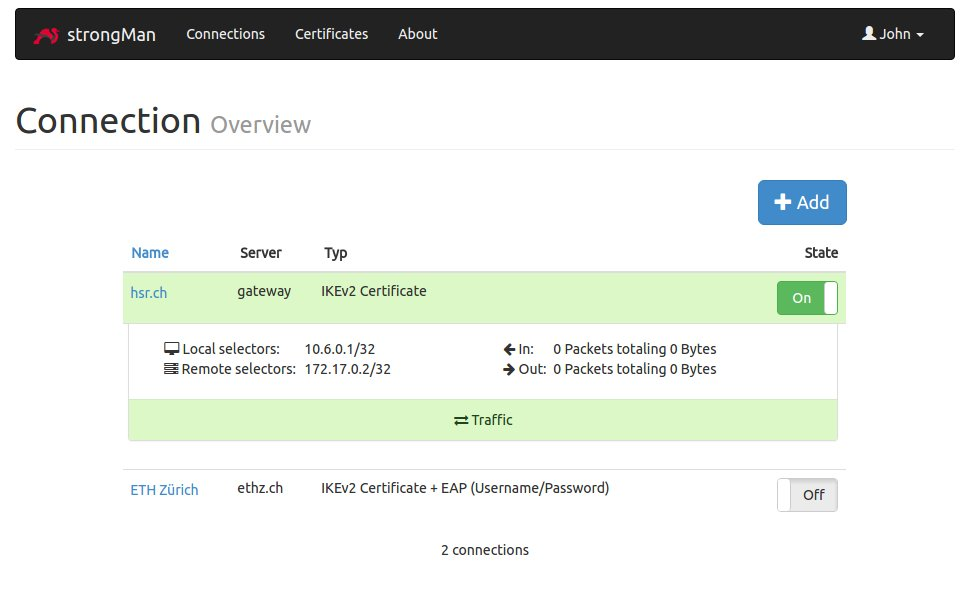
\includegraphics[width=440pt]{images/strongMan_einfuhrung.jpg}
\caption[strongMan Verbindungsübersicht]{strongMan Verbindungsübersicht}
\end{figure}